
\newcommand{\ctilde}{\raise.17ex\hbox{$\scriptstyle\mathtt{\sim}$}}

\documentclass{acm_proc_article-sp}
\usepackage{tikz}
\usepackage{pgfplots}
\usepackage[ruled, vlined ]{algorithm2e}
\usepackage{graphicx}
\usepackage{bera}% optional: just to have a nice mono-spaced font
\usepackage{listings}
\usepackage{xcolor}
\usepackage[T1]{fontenc}
\usepackage[utf8]{inputenc}
\usepackage{tabularx,ragged2e,booktabs,caption}
\newcolumntype{C}[1]{>{\Centering}m{#1}}
\renewcommand\tabularxcolumn[1]{C{#1}}

\colorlet{punct}{red!60!black}
\definecolor{background}{HTML}{EEEEEE}
\definecolor{delim}{RGB}{20,105,176}
\colorlet{numb}{magenta!60!black}

\lstdefinelanguage{json}{
    basicstyle=\normalfont\ttfamily,
    numbers=left,
    numberstyle=\scriptsize,
    stepnumber=1,
    numbersep=8pt,
    showstringspaces=false,
    breaklines=true,
    frame=lines,
    backgroundcolor=\color{background},
    literate=
     *{0}{{{\color{numb}0}}}{1}
      {1}{{{\color{numb}1}}}{1}
      {2}{{{\color{numb}2}}}{1}
      {3}{{{\color{numb}3}}}{1}
      {4}{{{\color{numb}4}}}{1}
      {5}{{{\color{numb}5}}}{1}
      {6}{{{\color{numb}6}}}{1}
      {7}{{{\color{numb}7}}}{1}
      {8}{{{\color{numb}8}}}{1}
      {9}{{{\color{numb}9}}}{1}
      {:}{{{\color{punct}{:}}}}{1}
      {,}{{{\color{punct}{,}}}}{1}
      {\{}{{{\color{delim}{\{}}}}{1}
      {\}}{{{\color{delim}{\}}}}}{1}
      {[}{{{\color{delim}{[}}}}{1}
      {]}{{{\color{delim}{]}}}}{1},
}


\begin{document}
\pagenumbering{arabic}

\title{Identifying Malicious Actors through Graph Analysis of DNS Chaff}
\subtitle{ STUNG (Stinger To Uncover Nefarious Garbage)}

\numberofauthors{5} 
\author{
\alignauthor
Michael Fields\\
%       \affaddr{Georgia Tech}\\
       \email{mfields7@gatech.edu}
\alignauthor
Trevor Goodyear\\
%       \affaddr{Georgia Tech}\\
       \email{tg@gatech.edu}
\alignauthor
Evan Stuart\\
%       \affaddr{Georgia Tech}\\
       \email{evan.stuart@gatech.edu}
\and % go to new row
\alignauthor
Brian Swenson\\
%       \affaddr{Georgia Tech}\\
       \email{bswenson3@gatech.edu}
\and % go to new row
\alignauthor
Mark Wisneski\\
%       \affaddr{Georgia Tech}\\
       \email{markwis@gatech.edu}
}

\date{19 April 2016}


\maketitle
\begin{abstract}
In this work, we apply graph metrics to an Active DNS dataset, provided by the Georgia Tech Astrolavos Lab, to characterize and identify malicious actors within the DNS infrastructure of the Internet. Active DNS uses a set of data sources -- including TLD Zone Files, public blacklists, and many others -- to gather approximately 250 million DNS records each day. We use A records from this dataset to form a graph. From this graph we derive various metrics for each vertex using the following algorithms: PageRank, betweenness centrality, kCore-decomposition, and in- and out-degree.

We propose a machine learning model derived from graph-based metrics for both quantifying and identifying which nodes within our Active DNS data set are malicious and we describe a system, STUNG (Stinger To Uncover Malicious Gambits), that supports the rapid generation of graph-based features for hundreds of millions data points using the streaming graph analysis platform STINGER.
\end{abstract}


\section{Introduction}


\begin{figure}[h]
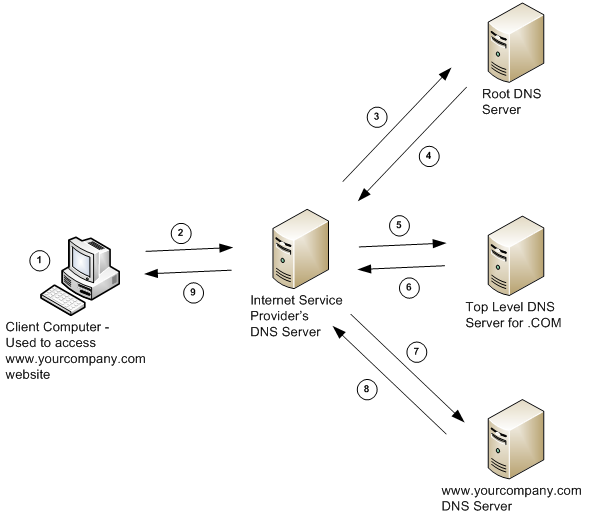
\includegraphics[width=0.5\textwidth]{images/DNS_basics.png}
\caption{Example of the Domain Name Resolution process \cite{DNS_fig}}\label{dns_diagram}
\end{figure}

The Domain Name System (DNS) \cite{rfc1034, rfc1035} maps domain names to IP addresses, and provides a core service to applications on the World Wide Web (WWW). Figure~\ref{dns_diagram} shows the DNS query cycle. Internet based attacks often leverage the use of DNS systems to mount attacks against unsuspecting users. For example, spywares exfiltrate user information to certain drop sites by using anonymously registered domains. Botnets make use of disposable domains to host malicious content or communicate with command and control servers and use the short life of the domains to avoid blacklisting. As a result, adversaries take advantage of the inherent agility, flexibility, and resilency of DNS in order to blend their malicious activities with that of benign DNS traffic, or DNS chaff.As malwares rely on domain names vis-a-vis IP addresses, DNS becomes indispensable in combating malwares. (e.g blacklisting, expired domains, et al.). By understanding and quantifying the nature of benign DNS chaff, we can then detect the characteristics of non-benign traffic and use that to track suspicious activities.

The threat landscape of the DNS infrastructure is constantly evolving and threat detection and classification mechanisms are becoming essential components of information security operations centers. An InfoBlox report notes that 74\%  of surveyed Chief Security Officers are actively seeking solutions that both facilitate the detection of malicious DNS activity and prevention of DNS outages.\cite{InfobloxPaper}

In 2005, Florian Weimar invented what is now called Passive DNS when he rebuilt the entire .de space one response at a time. Simply put, passive DNS is a system of record that stores DNS resolution data for a given location, record and time period. Since Weimar's work in 2005, security researchers have made significant progress in developing malicious DNS detection and mitigation technologies that leverage the passive DNS collection methods.  

This work uses a novel data set, active DNS, to derive security-relevant features using graph analysis and other analytic techniques. Unlike passive DNS data that is generated by user activity within a monitored network segment, active DNS data is collected by targeting specific domains and programatically performing DNS queries against the target set and recording the results. To summarize, active DNS collection methods allow researchers to observe and analyze DNS traffic that passive DNS collection methods would never produce.  

We introduce a system, STUNG: Stinger To Uncover Nefarious Garbage, to analyze DNS chaff and identify malicious actors using graph analysis and machine learning.

\subsection{TODO Outline the ML Process}

\section{BACKGROUND \& RELATED WORK}
The Astrolavos Lab at Georgia Tech developed a system whereby millions of domain names are queried several times during the day. Through this so-called Active DNS system, we are able to get a more-objective view of DNS entries than could be gleaned through Passive DNS. In Passive DNS, a system sits at a network boundary and records all DNS requests and responses. DNS can be very naturally represented as a graph in many different configurations. As the research into graph analytics begins to evolve, it is becoming increasingly popular to study attributes of DNS from a graph perspective.

\subsection{Related Work}
In this section we present related works from researchers who have studied aspects of DNS related to this work.

\subsubsection{GMAD}
In April 2014, Lee et. al. presented GMAD: Graph-based Malware Activity Detection, a system that uses graph analysis of DNS query patterns to detect malware activity. Graph features in this work include weakley-connected components, graph clustering, and blacklist matching~\cite{GMAD}.

\subsubsection{Notos}
Manos Antonakakis, Roberto Perdisci, David Dagon, Wenke Lee and Nick Feamster. "Building a Dynamic Reputation System for DNS", USENIX Security Proceeding of the 19th USENIX conference on Security, August 11-13, 2010

\subsubsection{Segugio}
Segugio is a system for analyzing passive DNS data from ISPs in order to detect malicious domains. It forms a bipartite graph of requester IP to resolved IP and derives several interesting features from this graph. The resulting graph is much denser than the graph constructed in STUNG. Segugio vertices had an average degree of \ctilde30, whereas STUNG vertices have an average degree of \ctilde2~\cite{Segugio}.


\section{Methodology}
Broadly, this work uses the open-source tools MongoDB and STINGER to store and query bulk Active DNS data and the Python library scikit-learn.

\begin{figure}[h]
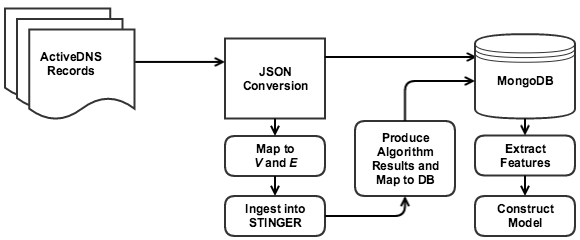
\includegraphics[width=0.5\textwidth]{images/stung_diagram_cropped.png}
\caption{System Architecture of STUNG}\label{fig:stung}
%\ref{fig:DNS}
\end{figure}

Table 1 lists the distribution of DNS query types present in one week of Active DNS data. In addition to these listed records, we see qtypes outside of the standard IANA qtype range. Future analysis of these non-standard qtypes may reveal interesting activities.


\begin{table}[h]
\centering
\caption{Distribution of qtypes}
\begin{tabular}{ |p{1.7cm}||p{1.7cm}|p{1.7cm}|p{1.7cm}|  }
\hline
%\multicolumn{4}{|c|}{Database Statistics} \\
 \hline
 {\bf Type ID}& {\bf IANA Name} & {\bf Percent Total}\\
 \hline
 2 & NS &  62.99\% \\
 \hline
 1 & A &  27.97\% \\
 \hline
 46 & RRSIG & 3.21\% \\
 \hline
 5 & CNAME &  2.27\% \\
 \hline
 6 & SOA &   1.716\% \\
 \hline
 50 & NSEC3 &  0.835\% \\
 \hline
 47 & NSEC &  0.650\% \\
 \hline
 43 & DS &  0.262\% \\
 \hline
 28 & AAAA&  0.104\% \\
 \hline
 16 & TXT& 26517& 0.002\% \\
 \hline
 41 & OPT& 5557& 0.000\% \\
 \hline
 39 & DNAME& 425& 0.000\% \\
 \hline
 15 & MC& 317& 0.000\% \\
 \hline
 3 & MD& 108& 0.000\% \\
 \hline
 12 & PTR& 90& 0.000\% \\
 \hline
 0 & N/A& 83 & 0.000\% \\
 \hline
 25 & KEY & 7 & 0.000\% \\
 \hline
 250 & TSIG & 7 & 0.000\% \\
\hline
\end{tabular}
\vspace{2mm}
Here we see the distribution of the top 18 qtypes observed within ActiveDNS records from 2016/01/26 to 2016/02/01.

\label{table:1}
\end{table}


\begin{figure}
\begin{lstlisting}[language=json,firstnumber=1]
{"type":"record",
  "name":"ActiveDns",
  "namespace":"astrolavos.avro",
  "avro.codec": "snappy",
  "fields":[
        {"name":"date","type":"string"},
        {"name":"qname","type":"string"},
        {"name":"qtype","type":"int"},
        {"name":"rdata","type":["string","null"]},
        {"name":"ttl","type":["int","null"]},
        {"name":"authority_ips","type":"string"},
        {"name":"count","type":"long"},
        {"name":"hours","type":"int"},
        {"name":"source","type":"string"},
        {"name":"sensor","type":"string"}]}";
\end{lstlisting}
\caption{ActiveDNS Record Schema}
\label{fig:my_label}
\end{figure}

% end of code to convey properties of our experiment


(MARK) Upon receiving the data we inquired on February 12th to better understand the data as some identification we anticipated was not present.  We inquired as to: 

''What was used to capture the data we received?''

''How can we get a description of the fields for the data?''

''Is there any difference between several directories?
More specifically, do they contain different sets of data or just different views of the same data?''
(MARK)


We worked hard to better understand the data.  For example at one point, we (MARK via Evan) looked at random choices and picked out random type of requests and there were 20 different DNS requests completely deprecated; not supported
(MARK via Evan)

(MARK via Evan)
We noticed there are all the different key types.  But does that make sense? We inputted a couple 100 million of them and ran queuies.  Tried to determine the qtypes.  Some were non-standardized.  For instance a qtype of 32-97645 (TTO) ??? Check this from my scribbles (TTO) which is the block that the standards body says for whatever kind of DNS request you want to make?  It is a custom style.  Could it be that the response values are just random hex values?  
(MARK via Evan)

Before we began data ingest we considered a possible of looking up temporary disposable domains. \cite{ManosbuildDNS}   For example, (MARK via Brain)
 you could take google.com, that was at the top, then you could make a graph of that then you would take like account.google.com then .google.com then you could just build a big tree with different nameservers in them.  This would comprise just one thing to do; perhaps not even requiring a graph (at least initially)
(MARK via Brian)

\subsection{Data Ingest}
In this section we detail our methods and performance characteristics for transforming data from the original AVRO files into formats that are amenable to processing.

(MARK)
We received an expired domains dataset (3.7GB of text) from acs-2 and uploaded to our VM.\cite{ChazdomainZ}  We continued to work on importing the active-dns dataset into Mongo.  This MongoDB installation uses the MMAPv1 DB engine.
(MARK)

We ingested data into ~5TB MongoDB collection.  However we aborted indexing as it was determined that it would take months to ingest.



\subsubsection{Graph Structure}


(MARK via Trevor)
A graph can be constructed that maps domain names -> IP addresses, with an edge type for each record type. Non-IP DNS records can be discarded for purposes of graph construction. This will at least allow us to see which domain names map to the same IP addresses. By making this a temporal graph, we can see changes in the graph. This data could conceivably be represented as: a single temporal graph, multiple static graphs, a static multigraph (multiple edges of the same type and direction between two nodes). Single temporal graph is easiest to work with but we lose duplicate edges. Multiple static graphs might be easiest to analyze and will accurately capture the contents of the entire dataset, but could be cumbersome to work with (lots of duplication). We have not worked much with multigraphs.  We will determine how easy they are to manipulate.
(MARK via Trevor)

Insert graphs using suitable LaTeX library here. Show both Domain to IP and Domain-IP-AuthorityIP graphs.

%Diagram
\begin{figure}
    \usetikzlibrary{arrows.meta}
    \begin{tikzpicture}
        \begin{scope}[every node/.style={circle,fill=blue!20}]
            \node (A) at (2.5,4) {QName};
            \node (B) at (2.5,1) {Rdata};
            \node (C) at (0,-1.5) [align=center] {Authority \\ IP 1};
            \node (D) at (2.5,-1.5) [align=center] {Authority \\ IP 2};
            \node (E) at (5,-1.5) [align=center] {Authority \\ IP N};
        \end{scope}
        
        \begin{scope}[>={Stealth[black]},
                      every node/.style={fill=white,circle},
                      every edge/.style={draw=black,very thick}]
            \path [->] (A) edge  (B);
            \path [->] (B) edge[bend right=20] (C); 
            \path [->] (B) edge (D); 
            \path [->] (B) edge[bend left=20] (E); 
        \end{scope}
    \end{tikzpicture}
\caption{
Example mapping of a single Active DNS A record to a set of edges and vertices.}
\label{fig:my_label}
\end{figure}



\subsubsection{STINGER}
STINGER is a, in-memory, community-developed, high performance, extensible data structure for dynamic graph problems which originated through the work of Georgia Tech researchers~\cite{STINGER}.

The idea to think bigger than conventional approaches (viz. statistical approaches) to analyzing DNS Chaff was inspired by a lecture given by Alex Beutel which we attended on February 26.\cite{LectureA} Large-graph modeler Beutel admitted that factorization was the tried and true method behind much of graph modeling.  But he wanted new tools to model his graphs so he could do it: 
in distributed fashion for scalability;
do it quickly;
do it in a flexible way;
At our very next team meeting, we began to contemplate the potential for new tools to help solve our modeling problem.
.
(MARK via Evan)
Our eureka moment hit when we considered putting the STINGER graph database to work.   STINGER does not have some properties but if we can get near instant analysis of the data as it came through, we make a data pipeline for it.  That could be beneficial.  One would expect that since this is a big set of data, you have to do statistics on order to scale to understand the structure of the data.  However STINGER offers a previous unexplored alternative.  Perhaps we would not even need a super model.  We could point to sections of the model that might be potentially useful because of the sheer volume of incoming data.

But if we could get real-time analysis as the data came in, it might be something useful; even just PageRank.


We envision being able to directly stream DNSCap data into both an archive (MongoDB) and the STINGER Graph Database. By doing so, we will have a dual pronged approach towards generating useful data models and graph metrics. For example, prominent features detected by the STINGER implementations of algorithms such as betweenness centrality and pagerank for a vertex could help us narrow down areas within the data archive to research. Significant variances from the norm for these metrics may be indicative of malicious behavior. We plan to build data models from the archival data and look for markers of that model in the real time stream that is constantly ingested into STINGER. Alerts from these systems would be displayed to an operational user through a web-based dashboard.


As the system developed, it operated as follows:
(MARK via Evan)

Data is inserted into STINGER through \textit{batches} which consist of many edges. We use the STINGER Python bindings and the \texttt{fastavro} Python package to read the Active DNS Apache AVRO files and construct a batch for each part file. In the dataset, each day of data is split into 600 parts, with each part file containing \ctilde 80MB of data or \ctilde 1.2M DNS records.

One day of valid A records is inserted into STINGER in approximately 14 hours. Following successful ingest, data analysis and reporting is very quick.


\subsubsection{MongoDB}
The first approach was to insert the entirety of this dataset into a MongoDB instance and perform analysis later. This is a common tactic in big data problems: push all data into a data lake and place the onus on data scientists later to figure out how to make sense of the data. This naive approach yielded a large datastore from which no actionable intelligence could be derived. We opted instead to ingest one day worth of data into a collection and to build from there. 

% TODO: Find TeX syntax to number paragraphs. subsubsubsection doesn't exist in sharelatex
\paragraph{Storage Engines}
MongoDB currently has three supported storage engines available to non-enterprise clients: MMAPv1, WiredTiger, and RocksDB. The first approach used MMAPv1, the oldest and most-stable engine. The next approach used RocksDB, a bleeding-edge key-value store used primarily in research applications by Facebook and only recently adapted for use with MongoDB. Finally, we use the WiredTiger storage engine, the latest engine officially supported by the MongoDB team. In both RocksDB- and WiredTiger-backed databases, we ensured appropriate indexes for fields which were likely to be frequently accessed or queried over.

We found RocksDB offered a marginal performance gain over MMAPv1 and WiredTiger but only when accessing date on flash storage. Ultimately, to ensure maximum read and write throughput we opted to store our data in memory using a ramdisk with the WiredTiger storage engine.


\subsection{Data Analysis}
In this work, we attempt to classify IPv4 addresses and domain names into two classes:
\begin{enumerate}
    \item Malicious
    \item Benign
\end{enumerate}  

\subsection{Classifier Selection}
We use traditional machine learning techniques to attempt classification of new hosts into one of these four categories.

\subsection{Features Used}


In this section we examine specific examples of our analysis finding interesting or malicious activity.


\subsubsection{PageRank}
PageRank is a popular influence metric for graph data. In a directed PageRank, nodes have high scores if 

\begin{figure}[ht!]
\centering
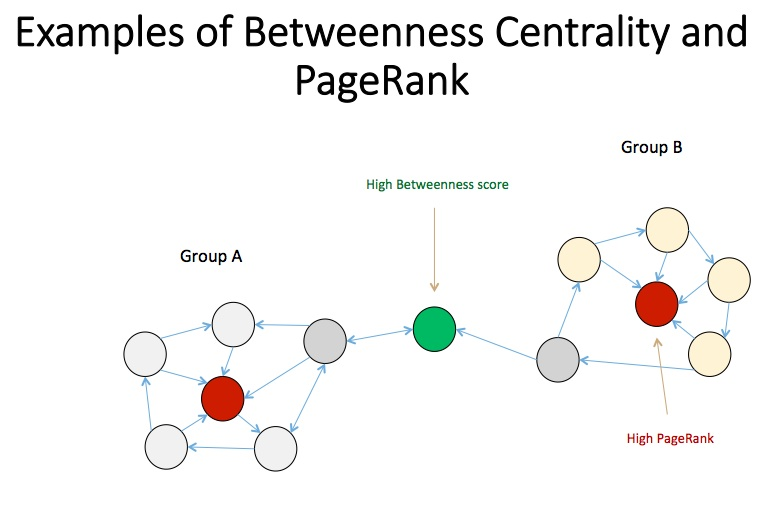
\includegraphics[width=60mm]{images/20160417 image ex of betweenes centrality and pagerank jpeg.jpg}
\caption{examples of Betweeness Centrality and PageRank \label{overflow}}
\end{figure}


\subsubsection{k-core}

(MARK via Trevor)
k-core clustering is common in graphs and simple clustering. Modularity-maximizing community detection can also be implemented for well-connected components.
(MARK via Trevor)

A $k$-core of a graph $G$ is a maximal connected subgraph of $G$ in which all vertices have degree at least $k$. Equivalently, it is one of the connected components of the subgraph of $G$ formed by repeatedly deleting all vertices of degree less than $k$. If a non-empty $k$-core exists, then, clearly, $G$ has degeneracy at least $k$, and the degeneracy of $G$ is the largest $k$ for which $G$ has a $k$-core.

The highest values of $k$-core belong to a cluster of IP addresses in southeast Asia, mostly China and Hong Kong. Reverse-resolving the top-indegree IPs show 

\begin{figure}[ht!]
\centering
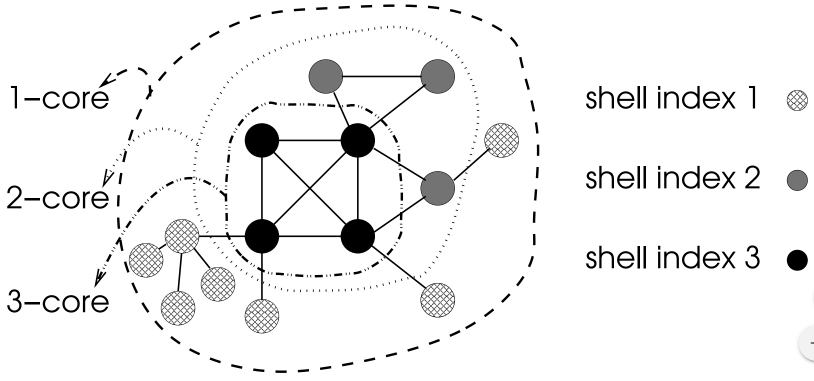
\includegraphics[width=70mm]{images/kcore.png}
\caption{Example showing $k$-core decomposition~\cite{alvarez2005k} \label{overflow}}
\end{figure}


\subsubsection{In-Degree}
This IP address, \texttt{69.172.201.208}, has the highest in-degree by an order of magnitude. Research indicates that this IP is from a provider of DoS-protection software names DOSarrest. \begin{figure}
\centering
    \usetikzlibrary{arrows.meta}
    \begin{tikzpicture}
        \begin{scope}[every node/.style={circle,fill=blue!20}]
            \node (A) at (0,4) {QName};
            \node (B) at (2.5,4) {QName};
            \node (C) at (5,4) {QName};
            \node (D) at (2.5,1) {Rdata};
        \end{scope}
        \begin{scope}[>={Stealth[black]},
                      every node/.style={fill=white,circle},
                      every edge/.style={draw=black,very thick}]
            \path [->] (A) edge[bend left=20]  (D);
            \path [->] (B) edge (D); 
            \path [->] (C) edge[bend right=20] (D); 
        \end{scope}
    \end{tikzpicture}
\caption{
Example of a RData with a high in-degree value.}
\label{fig:my_label}
\end{figure}




\subsubsection{Out-Degree}

\begin{figure}
\centering
    \usetikzlibrary{arrows.meta}
    \begin{tikzpicture}
        \begin{scope}[every node/.style={circle,fill=blue!20}]
            \node (A) at (2.5,4) {QName};
            \node (B) at (0,1) {Rdata};
            \node (C) at (2.5,1) {Rdata};
            \node (D) at (5,1) {Rdata};
        \end{scope}
        
        \begin{scope}[>={Stealth[black]},
                      every node/.style={fill=white,circle},
                      every edge/.style={draw=black,very thick}]
            \path [->] (A) edge[bend right=20]  (B);
            \path [->] (A) edge (C); 
            \path [->] (A) edge[bend left=20] (D); 
        \end{scope}
    \end{tikzpicture}
\caption{
Example of a QName with a high out-degree value.}
\label{fig:my_label}
\end{figure}

\subsubsection{Long Domain Names}


\section{RESULTS}
In this section we detail the the results of our described methodologies for Data Ingest and Analysis.

A first stop on the road to good detection analysis is: building detectors. A good detector is the one that has low false positives and high true positives. A ROC (receiver operating characteristic) curve was constructed to demonstrate we can perform such a measurement analysis for our detector.



\begin{figure}[ht!]
\centering
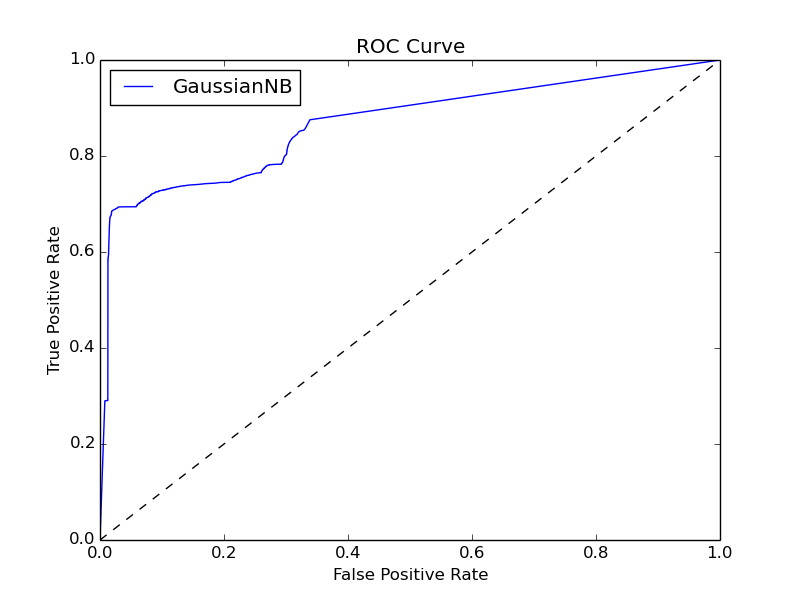
\includegraphics[width=90mm]{images/ROC.png}
\caption{Preliminary ROC Curve \label{overflow}}
\end{figure}

\begin{figure}[ht!]
\centering
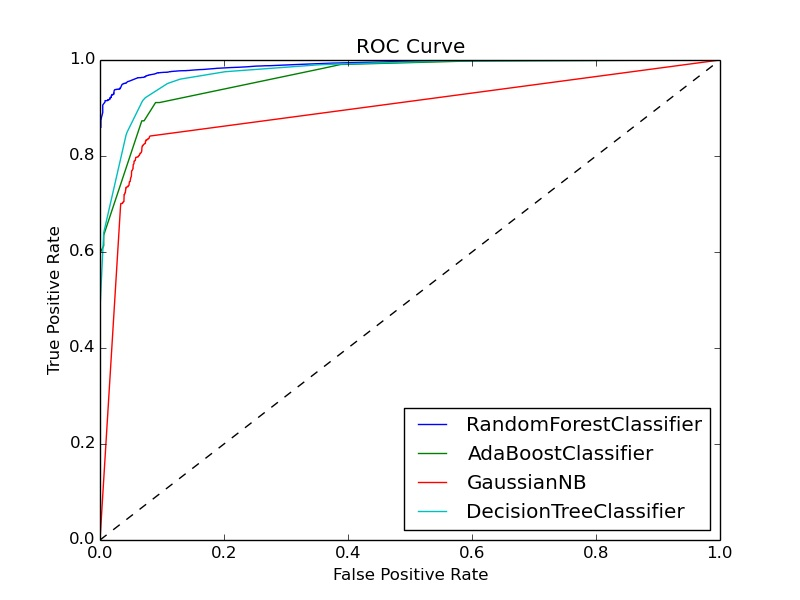
\includegraphics[width=90mm]{images/20160417_new_and_improved_ROC_jpeg.jpg}
\caption{New and Improved ROC Curve \label{overflow}}
\end{figure}


\begin{table}[h]
\centering
\begin{tabular}{ |p{3.5cm}||p{2cm}|  }
 \hline
 TP Rate& 85.89\%\\
 FP Rate& 14.11\%\\
 Accuracy & 83.14\%\\
 Precision & 85.05\%\\
 Recall& 80.39\%\\
\hline
\end{tabular}
\vspace{2mm}
\caption{Random Forest Classifier Statistics}
\label{table:2}
\end{table}

\begin{table}[h]
\centering
\caption{Feature Importance}
\begin{tabular}{ |p{3.5cm}||p{2cm}|  }
 \hline
 avg\textunderscore ip\textunderscore bc& 31.88\%\\
 avg\textunderscore ip\textunderscore bctf&8.17\%\\
 avg\textunderscore ip\textunderscore in & 30.28\%\\
 avg\textunderscore ip\textunderscore kn& 31.88\%\\
 avg\textunderscore ip\textunderscore out& 31.88\%\\
 avg\textunderscore ip\textunderscore pr& 31.88\%\\
 avg\textunderscore ip\textunderscore wccs& 31.88\%\\
 max\textunderscore ip\textunderscore bc& 31.88\%\\
 max\textunderscore ip\textunderscore bctf&8.17\%\\
 max\textunderscore ip\textunderscore in & 30.28\%\\
 max\textunderscore ip\textunderscore kn& 31.88\%\\
 max\textunderscore ip\textunderscore out& 31.88\%\\
 max\textunderscore ip\textunderscore pr& 31.88\%\\
 max\textunderscore ip\textunderscore wccs& 31.88\%\\
 min\textunderscore ip\textunderscore bc& 31.88\%\\
 min\textunderscore ip\textunderscore bctf&8.17\%\\
 min\textunderscore ip\textunderscore in & 30.28\%\\
 min\textunderscore ip\textunderscore kn& 31.88\%\\
 min\textunderscore ip\textunderscore out& 31.88\%\\
 min\textunderscore ip\textunderscore pr& 31.88\%\\
 min\textunderscore ip\textunderscore wccs& 31.88\%\\
 dom\textunderscore bc&8.17\%\\
 dom\textunderscore bctf&8.17\%\\
 dom\textunderscore in & 30.28\%\\
 dom\textunderscore kn& 31.88\%\\
 dom\textunderscore out& 31.88\%\\
 dom\textunderscore pr& 31.88\%\\
 dom\textunderscore wccs& 31.88\%\\
\hline
  
\end{tabular}
\vspace{2mm}
\label{table:2}
\end{table}



\subsection{Data Ingest}

\subsubsection{STINGER}
For one day of non-null A records, STINGER ingested 138,299,998 vertices and 198,290,487 edges over a timespan of 17.78 hours, averaging 3097 edges/second over that timespan. As seen in the graph below, ingest performance of STINGER is exponentially proportional to its runtime.

\begin{figure}[ht!]
\centering
\begin{tikzpicture}
\begin{loglogaxis}[
    title={Ingest rate of A Records into STINGER},
    xlabel={Elapsed Hours},
    ylabel={Edges per second},
    xtick={0,0.01,0.1,1,10,50},
    ytick={0,10,100,1000,10000,100000,1000000,10000000},
    ymajorgrids=true,
    grid style=dashed
]
\addplot[
    color=blue,
    mark=*,
    mark options={%
        scale=0.5
    }
    ]
    table{stinger_ingest_hours.csv};
 
\end{loglogaxis}
\end{tikzpicture}
\caption{Ingest rate into STINGER for 20160126 \label{overflow}}
\end{figure}

\paragraph{Non-Uniform Memory Access}
The primary machine running STINGER for this analysis consists of four Intel Xeon E7-4880 v2 CPUs with 1TB main memory. This machine seemed at first to be the perfect candidate for large memory-dependant applications such as STINGER. However, in practice random memory access across QPI for four sockets creates much more overhead. Compounding this issue was a bad DIMM in one of the memory controllers, causing many ECC interrupts. Confining STINGER to run on two sockets and their respective memory controllers increased ingest rates dramatically as seen below.


\subsubsection{MongoDB}
MongoDB served as the backing datastore for processed AVRO records, providing a convenient platform for data retrieval, query, simple analysis, and storage of engineered features. On the recommendation of many online sources, we moved forward using the RocksDB storage engine to ingest seven days of AVRO records.

\begin{figure}[ht!]
\centering
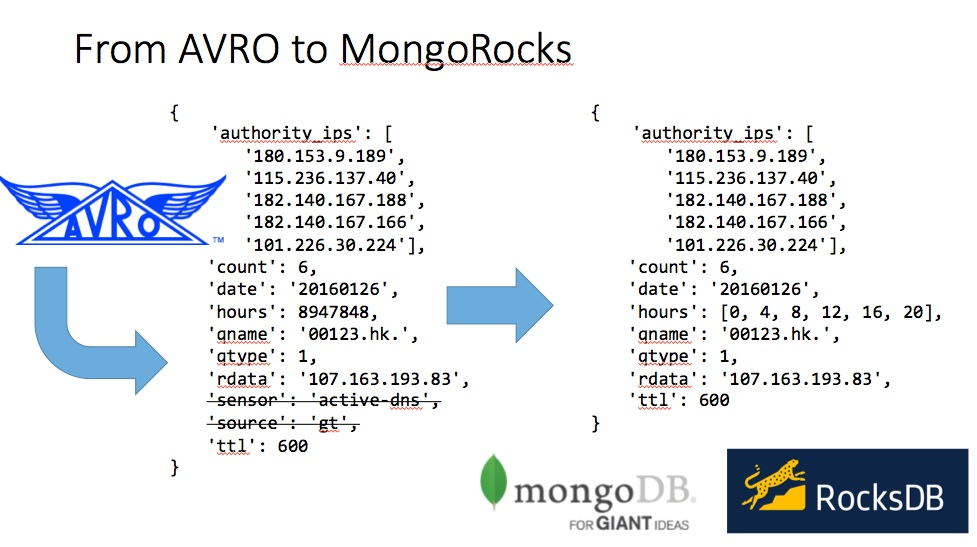
\includegraphics[width=90mm]{images/20160417 image AVRO to MongoRocks jpeg.jpg}
\caption{AVRO to MongoRocks \label{overflow}}
\end{figure}


RocksDB averaged 5567 processed records per second.

WiredTiger averaged 36608 processed records per second, and includes Full-Text indexes for qname. In contrast to the other attempted storage engines, this ingest attempt used only A records from one day. RocksDB and MMAPv1 used all qtypes and spanned multiple days.

\paragraph{}

\subsection{Data Analysis}
We did math and it went really well. We couldn't believe it worked either.

(TTO)

SHOW ENOUGH GENERIC TESTING MODEL SELECTION  use widely uses algos and see what you can do with them

%to add generic testing to avoid personal bias
\begin{figure}[ht!]
\centering
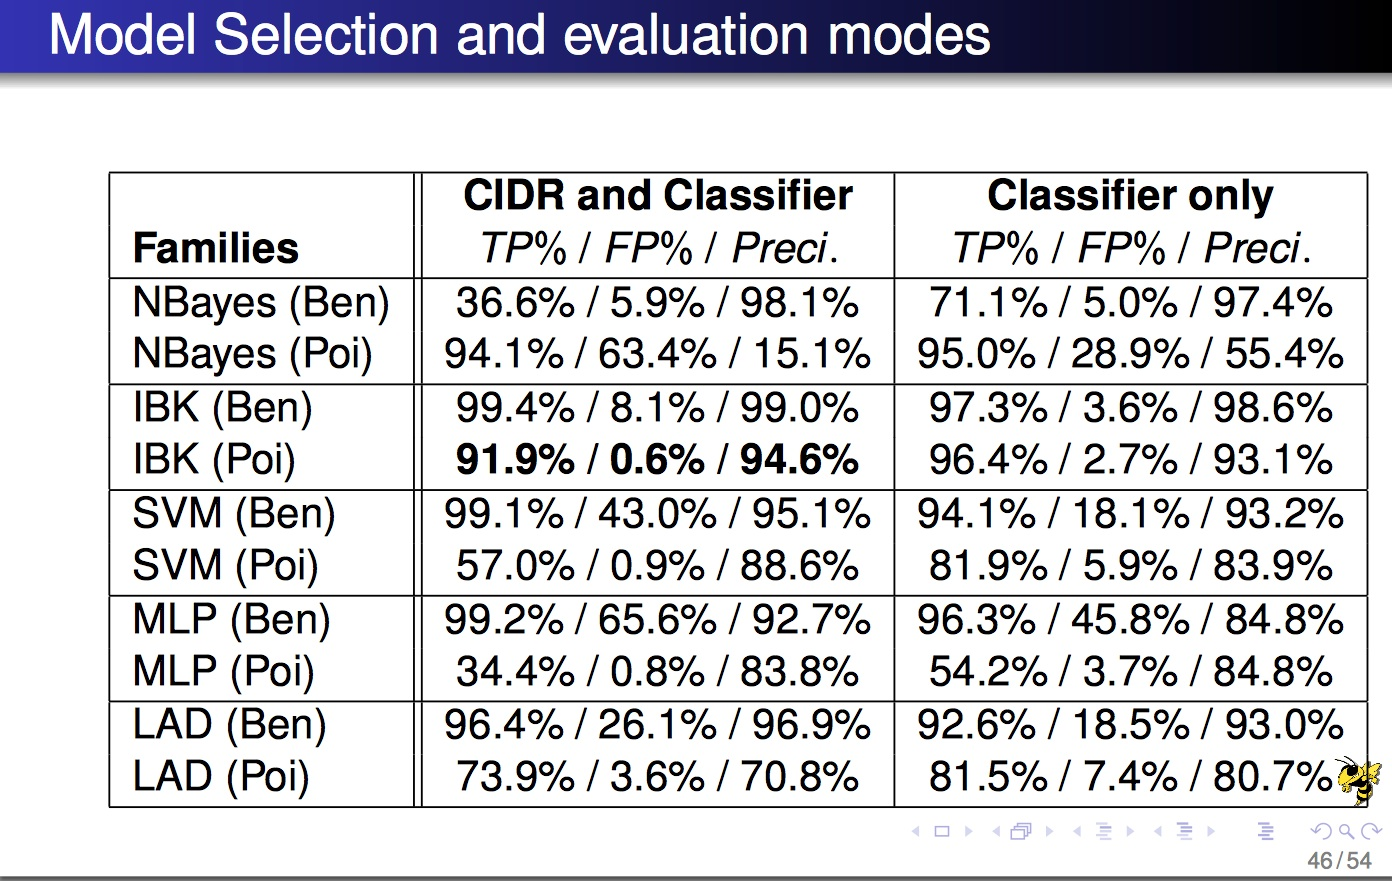
\includegraphics[width=70mm]{images/20160417 image show generic testing to avoid personal bias jpeg.jpg}
\caption{generic testing used to avoid perosnal bias \label{overflow}}
\end{figure}

% end of code showing generic testing to avoid personal bias
(TTO)


Maybe we can put in a chart of RocksDB, MMAPv1 and WiredTiger here as our "generic testing to demonstrate we are "not using personal bias"


\section{FUTURE WORK}


\subsection{Authority Quantification}
We posit that authorities in the DNS graph maintain relatively constant values, especially from day to day. Furthermore, highly-authoritative hosts should be well-known: for example Google, Hurricane Electric, TLD roots, etc. Additionally, authoritative IPs should be in trusted Autonomous Systems and reverse-lookup of authoritative IPs should result in domain names which are not on public blacklists and which have domain names in the same subnet with a high string-similarity score. We present a method by which 

\subsection{Finding Malignity through Degree Metrics}
Another interesting aspect of the graph that can be explored is the degree metrics of domain names and their resolved IPs. For web publishing platforms such as Tumblr or Blogger, each user's blog is granted a unique DNS entry, for example \texttt{cs6262.tumblr.com}. It is expected behavior for a large number of domains for these services to point to a very small number of IPv4 addresses. However, if domain names with a low degree of similarity point to the same IP address, this may be indicative of malicious activity.

Although malware infections cannot occur in an instant as domain names related with malware have to go through the malware and propagation stage \cite{Manos2012Auth}, we still expect to act quickly.

(MARK via Trevor)
We can characterize nodes which exhibit certain behaviors based on their properties. For instance, perhaps an IP address with a lot of domain names pointing to it is likely to experience greater churn than IPs with smaller numbers of records. We presume the graph will not be well-connected, forcing us to characterize on relatively simple metrics (We will focus on ''degree'' if the largest WCC is a small fraction of the graph)
(MARK via Trevor)

Thus we will begin with the notion that nodes within our graph with abnormally high in-degree or out-degree values are indicators of malicious activity.

\subsection{DNS Health Check}
Finally, we use metrics of the total graph to compute characteristics about the state of DNS (in terms of A Records) for each day. This includes statistics such as graph diameter, total number of in-edges, out-edges, vertices, edges

\subsection{Technologies to Explore}

\subsubsection{Graph Analytic Platform}
The Berkeley Graph Algorithm Platform (GAP) Project is an effort through David Patterson's group at the University of California -- Berkeley to accelerate graph algorithms through software optimization and hardware acceleration~\cite{GAP}. 

GAP is likely a more appropriate tool for static graphs such as the Active DNS dataset than STINGER. GAP uses Compressed Sparse Row format to store the graph in a very efficient manner. Much research has been done in this field to prove the performance and efficiency characteristics of CSR notation. STINGER does not use CSR format, it instead uses an internal data structure which is optimized for streaming graphs -- CSR graphs are typically immutable once established.

\subsubsection{Redis}
Many graph engines, including STINGER and GAP, most-efficiently perform graph ingest on flat files using the Edge List (EL) format. In this format, a graph is specified with one edge on each line of a text file, with integers for vertex IDs specifying the source and destination for each edge. In order to efficiently map domain name and IP address strings, we explored using the Redis key-value store. By using the edge list mapping we hoped to avoid the need to store the full text of domain names in our graph which could be dozens of characters long, which at scale has significant impact on our graph's memory footprint.

To effectively map a vertex's plain text content to an integer value, we determined a bi-directional hash-map as seen in figure? to be the most efficient means of accomplishing the mapping.
Unfortunately we achieved a maximum throughput of \ctilde 2,000 actions per second using this method. STINGER's lowest rate of ingest was \ctilde 6,000 edges per second, so we found this method of string factorization unsuitable.

\begin{algorithm}
\SetAlgoLined
\KwResult{ Bi-Directional mappping of domains/IPs and vertex IDs }
\tcc{Init hash-map keyed on domain/IP values}
 $dH \leftarrow initHashMap$\\
\tcc{Init hash-map keyed on vertex IDs}
 $vH \leftarrow initHashMap$\\
 \tcc{Init atomic counter for vertex ID}
 $vID \leftarrow 0$\\
 \For{Record in DataSet}{
  $Qname \leftarrow Record[qname]$\\
  $Rdata \leftarrow Record[rdata]$\\
  $Source \leftarrow dH(Qname)$\\
  $Dest \leftarrow dH(Rdata)$\\
  \If{Source is Null}{
   $dH(Qname) \leftarrow vID$\\
   $vH(vID) \leftarrow Qname$\\
   $Source \leftarrow vID$\\
   $vID \leftarrow vID + 1$\\
   } 
   \If{Dest is Null}{
   $dH(Rdata) \leftarrow vID$\\
   $vH(vID) \leftarrow Rdata$\\
   $Dest \leftarrow vID$\\
   $vID \leftarrow vID +1$\\
   }
   {insertStinger(Source, Dest)}\;
 }
\caption{Bi-Directional Redis Hash Map}
\end{algorithm}



\section{CONCLUSIONS}

(TTO)
How do the aforementioned ideas connect to what we discussed in class, or to what scholars have written in their treatment of the topic? Vixie? Dagon? Manos?

What new ideas do we add to the conversation? 
What ideas are critiqued?  Get cleaner data sets next time??

What are the limitations of the data, methods, or results? 2 weeks of data??
What are the consequences of the strongest idea that comes out of your paper?

Can we return to the question or situation described in your introduction? e.g. Manos always returns from his DNSSEC angle back to Kaminski
(TTO)

 
 
Researchers (e.g. Vixie, Antonakakis, Dagon, et al.) have gone above the call of duty to trumpet the importance DNS security to the community.\cite{LectureB}  What we have done is gone one step further to arm security researchers with a system have flaunts the potential to add previously unseen speed in analyzing incredibly large data sets.

Whether our progress to this point was serendipitous or just lucky, the fact remains that research cannot stop here.  Our conversations with the researchers at Astroslavos and amongst ourselves reinforces the need for more research.

More specifically, the data utilized in this project contained inconsistent identification which slowed our progress.  That obstacle exists no more as the Astroslavos Lab now utilizes more detailed data.  In addition, our work in this paper spanned only a two week period.  Longer testing periods might yield new insights.

Discounting the chances of ubiquitous DNSSEC to protect DNS in the future, our experience of trying unorthodox methods to improve DNS security could among the better options for researchers in the field. 

We understand to need to improve STUNG as the Astroslavos Lab (our data source) expressed a desire to continue to grow.  That is to say they have over three times the data with better domain visibility and more types than they had six months ago.  We will need to keep up with or exceed their pace.   

Our meeting at the Astroslavos Lab concluded with high expectations for the next steps: "The whole point of this paper was not to do something for one class but also to continue thinking about these things.  We'll think of possible future projects beyond the class.  Our work will intersect with the other stuff."  Indeed, it is a matter of time until we suppose the nefarious operators will read this paper and plot to improve their attacks.  We must continue to improve our system.



\section{ACKNOWLEDGEMENTS}


Silo Busting in Information Security: The SIE Approach, Paul Vixie, Location:Belinda InterContinental KL, Kuala Lumpur, Malaysia , Time: 9-10 A.M., October 11, 2012

Seminar: Beyond Who and What: Answering How? And Why? By Modeling Large Graphs, Alex Beutel, Location: Klaus 2447, Time: 10-11 A.M., February 26, 2016

STUNG team interview at Astroslavos, Athanasios Kountouras, Yacin Nadij, Chaz Lever, Location: Klaus 3112, 3-4 P.M., March 23, 2016


\paragraph{}


\bibliographystyle{unsrt}
\bibliography{references}



\end{document}
